\documentclass[a4paper, 11pt]{article}
\addtolength{\hoffset}{-1cm}
\addtolength{\textwidth}{2cm}
\usepackage[utf8]{inputenc}
\usepackage[frenchb]{babel}
\usepackage[T1]{fontenc}

%\usepackage[bottom]{footmisc}

\usepackage{multicol}
\usepackage{listings}
\usepackage{graphicx}
\usepackage{hyperref}
\usepackage{amssymb}
\usepackage{amsmath}

\usepackage{color}
\definecolor{lightgray}{rgb}{.9,.9,.9}
\definecolor{darkgray}{rgb}{.5,.2,.2}
\definecolor{purple}{rgb}{0.65, 0.12, 0.82}
\definecolor{brown}{RGB}{140, 0, 0}

\lstnewenvironment{OCaml}
                  {\lstset{
                      language=[Objective]Caml,
                      breaklines=true,
                      showstringspaces=false,
                      commentstyle=\color{red},
                      stringstyle=\color{darkgray},
                      identifierstyle=\ttfamily,
                      keywordstyle=\color{blue},
                      basicstyle=\footnotesize,
                      escapeinside={/*}{*/},
                      %xleftmargin=0.08\textwidth
                    }
                  }
                  {}
\lstnewenvironment{OCamlEx}
                  {\lstset{
                      language=[Objective]Caml,
                      breaklines=true,
                      showstringspaces=false,
                      commentstyle=\color{red},
                      stringstyle=\color{darkgray},
                      identifierstyle=\ttfamily,
                      keywordstyle=\color{blue},
                      basicstyle=\footnotesize,
                     escapeinside={/*}{*/},
                      frame=single,
                      numbers=left,
                      %xleftmargin=0.08\textwidth
                    }
                  }
                  {}
\newcommand{\class}{\ttfamily\textit{class}}
\newcommand{\interface}{\ttfamily\textit{interface}}
\newcommand{\name}{\ttfamily\textit{name}}
\newcommand{\package}{\ttfamily\textit{package}}
\newcommand{\ident}{\footnotesize\textbf{ident}}
\newcommand{\fun}[1]{\ttfamily\textbf{#1}}

\lstdefinelanguage{idlgrammar}{
  morekeywords={package,abstract,extends,class,implements,static,final,<ini>,interface,callback,array,[,],{,},
    name ,void,boolean,byte,char,short,int,long,float,double,string},
  alsoletter=[]{},
}
\lstnewenvironment{idl}
                  {\lstset{
                      language=idlgrammar,
                      breaklines=true,
                      showstringspaces=false,
                      keywordstyle=\ttfamily\color{blue},
                      identifierstyle=\ttfamily\textit,
                      basicstyle=\footnotesize,
                     escapeinside={(*}{*)},
                      %xleftmargin=0.08\textwidth
                    }
                  }
                  {} 
\lstnewenvironment{idlEx}
                  {\lstset{
                      language=idlgrammar,
                      breaklines=true,
                      showstringspaces=false,
                      commentstyle=\color{red},
                      stringstyle=\color{darkgray},
                      identifierstyle=\ttfamily\textit,
                      keywordstyle=\color{blue},
                      basicstyle=\footnotesize,
                     escapeinside={/*}{*/},
                      frame=single,
                      numbers=left,
                      %xleftmargin=0.08\textwidth
                    }
                  }
                  {}

\lstnewenvironment{javaEx}
                  {\lstset{
                      language=Java,
                      breaklines=true,
                      showstringspaces=false,
                      commentstyle=\color{red},
                      stringstyle=\color{darkgray},
                      identifierstyle=\ttfamily\textit,
                      keywordstyle=\color{blue},
                      basicstyle=\footnotesize,
                     escapeinside={/*}{*/},
                      frame=single,
                      numbers=left,
                      %xleftmargin=0.08\textwidth
                    }
                  }
                  {}


\newcommand{\camljava}{{\tt{camljava}}}

%%%%%%%%%%%%%%%%%%%%%%%%%%%%%%%%%%%%%%%%%%%%%%%%%%%%%%%%%%%%%%%%%%%%%%%%%%%%%%



\title{\vfill
  \huge L'interopérabilité entre OCaml et Java\\
}
\author{
  Béatrice Carré \\
  beatrice.carre@etu.upmc.fr \\
  \\
  Encadrants : Emmanuel Chailloux, Xavier Clerc et Grégoire Henry \\
}
\date{\today\vfill}

\begin{document}

\maketitle
\newpage
\tableofcontents
\newpage

\section*{Introduction}
\addcontentsline{toc}{section}{Introduction}
Il est utile de réutiliser dans un certain langage du code
écrit dans un autre, sans avoir à le réécrire.
Il arrive souvent de vouloir utiliser l'expressivité et
l'élégance du langage Ocaml autant que le style objet de Java et la
diversité de son API.

C'est pourquoi l'interopérabilité est un problème intéressant.
Mais elle engendre beaucoup de questions sur la gestion de
plusieurs éléments :
la cohérence des types d'un langage à l'autre,
la copie ou le partage des valeurs d'un monde à l'autre,
le passage des exceptions,
la gestion automatique de la mémoire (GC\footnote{Garbage Collector}), 
et des caractéristiques de programmation qui ne sont pas forcément gérées par les
deux langages.

OCaml et Java comportent des différences entre leurs modèles
objet, comme le montre le tableau ci-dessous, il donc est nécessaire
de réduire l'étude à leur l'intersection.

\medskip
\noindent
\begin{tabular}{|l|c|c|c|c|}
  \hline
  \emph{caractéristiques} & \emph{Java} & \emph{OCaml} \\
  \hline
  accès champs & selon la visibilité & via appels de méthode\\\hline
  variables/méthodes statiques & \checkmark & fonctions/décl. globales\\\hline
  typage dynamique & \checkmark & $\times$ \\\hline
  surcharge & \checkmark & $\times$ \\\hline
  héritage multiple & seulement pour les interfaces & \checkmark\\
  \hline
\end{tabular}

\medskip
Deux travaux ont déjà été réalisés pour l’interopérabilité entre
OCaml et Java à travers leur modèle object respectif :
\begin{itemize}
\item \emph{O’Jacaré}\cite{O'Jacaré} conserve les runtimes des deux langages (GC,
Exceptions, ...) et les fait communiquer par l'interface \camljava \cite{camljava},
avec l'aide de classes encapsulantes générées par O'Jacaré.

\item \emph{OCaml-java
  2.0}\cite{OCaml-Java} utilise un seul runtime, en compilant code le OCaml en byte-code
Java. La manipulation des classes Java se fait à l'aide de nouveaux types introduits.
\end{itemize}
L'idée est de profiter des deux approches : d'une part, d'un accès simple à des classes
définies, en générant grâce à O'Jacaré le code nécessaire à cet accès 
et profiter d'autre part de l'accès direct à toute
l'API Java en ne gardant qu'un seul runtime, la
JRE, grâce à \emph{OCaml-Java}

Après l’étude des deux outils, le projet consiste à engendrer pour
ocaml-java les fichiers d’encapsulation d'O’Jacaré. Ce
portage est réalisé en OCaml étant donné qu'il reprend ce qui
a déjà été développé pour O’Jacaré. Cette adaptation ne gère pas les appels de Java vers OCaml (\emph{callback}\footnote{attribut représentant le sens d'appel de Java vers OCaml}).
\newline

Dans ce rapport, nous décrivons le schéma global d'O'Jacaré, et d'Ocaml-Java
pour en faire ressortir les avantages d'un portage d'O'Jacaré (O'Jacaré 2) pour \emph{OCaml-Java}.
Nous détaillons par la suite les modifications apportées à la
génération d'interfaces, adaptée pour une encapsulation utilisable par
le compilateur d'\emph{OCaml-Java}.
Pour finir, un exemple d'application sera présenté.
\newpage









\section{L'interopérabilité entre OCaml et Java}

%%%%%%%%%%%%%%%%%%%%%%%%%%%%%%%%%  1.1  O'Jacaré   %%%%%%%%%%%%%%%%%%%%%%%%%%%%%%%%%%%

\subsection{O'Jacaré, un générateur de code d'interface}

\subsubsection{Principe global}
O'Jacaré génère le code nécessaire à l'encapsulation des classes
définies dans un IDL\footnote{Langage de définition d'interface}, pour permettre aux interfaces avec C de chacun des deux langages de communiquer.

Lorsqu'on parle d'une classe encapsulante (capsule) d'une classe Java, 
on parle d'une classe OCaml qui porte une référence sur l'objet Java en question,
et qui est chargée de faire les opérations sur celui-ci.

L'appel à des classes et méthodes Java est alors possible en appelant
les méthodes de la capsule générée, qui va gérer l'appel aux classes
Java par le biais de l'interface \camljava.
Le code Java généré pour le callback va permettre avec le même
principe, les appels dans l'autre sens.

\camljava est une interface bas-niveau basée sur les interfaces de chaque langage avec C : la JNI\footnote{Java Native Interface} et \emph{External}.

La génération de code se fait en plusieurs passes :
\begin{itemize}
\item analyse lexicale et analyse syntaxique de l' IDL donnant un AST.
\item vérification des types de l'AST, donnant un nouvel arbre CAST\footnote{Pour \emph{Checked AST}}.
\item la génération des fichiers Java nécessaires pour un appel callback. 
\item la génération à partir du CAST des classes encapsulantes dans un fichier .ml
\item la génération à partir du CAST du module .mli adapté
\end{itemize}
Les deux dernières étapes seront présentées plus en profondeur dans la
section \ref{2.1}.
Un schéma décrit ces étapes dans la figure 2. 

%% \begin{figure}[h]
%%   \centering
%%   \includegraphics{schemaOjacare.pdf}
%%   \caption{Schéma global de la génération d'O'Jacaré}
%% \end{figure}



\subsubsection{Génération de code}
La génération de code se fait à partir d'un IDL, dont la grammaire
(BNF\footnote{Backus-Naur Form}) est définie en annexe dans la section \ref{4.1}.
Dans cet IDL, nous pouvons définir des déclarations qui sont à
l'intersection de ce qui est accessible dans les modèles objet de
chaque langage. 

Le but de cet IDL est de définir la signature des
classes Java déjà définies, que nous voulons manipuler du côté OCaml.
Ces classes encapsulantes servant à faire le lien entre les
classes/interfaces de chaque côté, il n'est donc nécessaire de définir
dans l'IDL que les méthodes que nous voulons appeler depuis OCaml.

Voici un exemple de déclarations dans un IDL, si on veut utiliser la classe Point définie à gauche. Il n'est nécéssaire de définir dans l'IDL uniquement les méthodes ou attributs que l'on veut manipuler depuis OCaml.


\begin{multicols}{2}
Point.java
\begin{javaEx}
  package mypack;
  public class Point {
    int x;
    int y;
    public Point() { 
      this.x = 0;
      this.y = 0;
    }
    public Point(int x,int y) {
      this.x = x;
      this.y = y;
    }
    public void moveto(int x,int y){
      this.x = x;
      this.y = y;
    }
    public String toString() {
      return "("+x+","+y+")";
    }
    public double distance() {
      return Math.sqrt
      (this.x*this.x+this.y*this.y);
    }
    public boolean eq(Point p) {
      return this.x == p.x 
          && this.y == p.y;
    }
  }
\end{javaEx}

\bigskip

point.idl
\begin{idlEx}
package mypack;
class Point {
  int x;
  int y; 
  [name default_point] <init> ();
  [name point] <init> (int,int);
  void moveto(int,int);
  string toString();
  boolean eq(Point);
}
\end{idlEx}

Pour une déclaration de classe ou interface, la génération de code
donne :
\begin{itemize}
  \item Un type abstrait correspondant au type Java
  \item Un type classe t
  \item Une classe encapsulante C de type t
  \item 1 à n classes Ci, sous-classes de C (une par constructeur),
 
    0 si c'est une interface
  \item Une fonction instanceof pour ce type
  \item Une fonction de cast pour ce type
\end{itemize}

\ 
\newline

\bigskip

\end{multicols}
Vous trouverez en annexe le code du fichier généré par ces déclarations.

Les fichiers générés sont destinés à être compilés avec l'aide la bibliothèque
\camljava.

\subsubsection{Compilation avec la bibliothèque \camljava}
\camljava gère l'interfacage entre OCaml et Java via C.

Un exemple d'utilisation de cette bibliothèque est :
\begin{OCamlEx}
let clazz = Jni.find_class "mypack/Point" in
let id = Jni.get_methodID clazz "<init>" "(II)V" in
let java_obj = Jni.alloc_object clazz : Jni.obj in
Jni.call_nonvirtual_void_method java_obj clazz id 
          [| Jni.Camlint 1; Jni.Camlint 2 |];;
\end{OCamlEx}

Les références sur les objets Java correspondent à un type abstrait en
OCaml, dans lequel des opérations donnent accès à des méthodes ou à des
champs de cet objet Java. 

L'exécution se fait dans les 2 runtimes, qui peuvent alors communiquer.

La gestion des exceptions est faite par encapsulation aussi, et la
gestion de la mémoire se fait par une mise en racine de l'objet dans la mémoire
l'autre monde avant de le passer en référence.

Mais cette gestion avec deux Garbage Collector et deux ensembles de racines pour la mémoire reste incertaine, dans la mesure où 
du point de vue mémoire tout objet Java alloué en O’Caml est une
racine du GC de Java. Quand O’Caml ne l’utilise plus, la racine Java
est supprimée mais l’objet peut être conservé par le GC de Java s’il
est référencé par un autre objet encore vivant. On retrouve
donc les problèmes inhérents aux compteurs de références pour les
structures circulaires.



\begin{figure}[h]
  \centering
  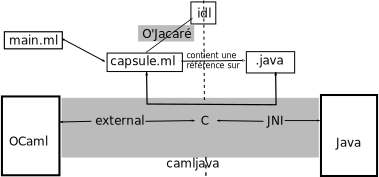
\includegraphics{schemaCamljava2.pdf}
  \caption{La communication grâce à \camljava}
\end{figure}









%%%%%%%%%%%%%%%%%%%%%%%%%%%%%%%%%  1.2  \emph{OCaml-Java}   %%%%%%%%%%%%%%%%%%%%%%%%%%%%%%%%%%%

\subsection{\emph{OCaml-Java} : compilation de code OCaml vers du bytecode Java}

\subsubsection{Principe global}

\emph{OCaml-Java} est un compilateur, générant du code octet Java (.jar) à
partir d'un programme OCaml. Ce processus s'effectue en deux phases :
\begin{enumerate}
\item La compilation vers du code intermédiaire 
\item La résolution dynamique pour produire un exécutable pour la
  JVM\footnote{Java Virtual Machine}
\end{enumerate}
Il est naturellement possible d'utiliser des bibliothèques Java en
utilisant la barrière d'abstraction d'\emph{OCaml-Java}.

\begin{figure}[h!]
  \centering
  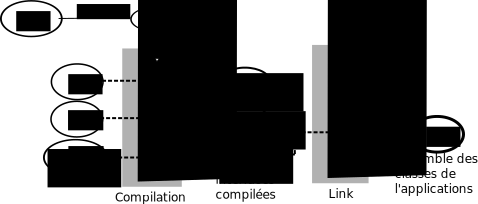
\includegraphics{schemaOCamlJava.pdf}
  \caption{Schéma global du compilateur d'\emph{OCaml-Java}}
\end{figure}

\newpage
\subsubsection{Barrière d'abstraction : manipuler du Java}
\noindent
Description des types manipulés par \emph{OCaml-Java} permettant un accès au
monde de Java depuis celui d'OCaml :

\begin{tabular}{|l|l|}
  \hline
  \emph{types OCaml-Java} & \emph{descriptions et exemples} \\\hline
  java\_instance & référence sur une instance Java  \\
  \hline
  java\_constructor & signature d'un constructeur  \\
  &  "java.lang.Object()" \\
  \hline
  java\_method & signature d'une méthode \\
  & "java.lang.String.lastIndexOf(String):int"\\
  \hline
  java\_field\_get & signature d'un attribut\\
  & "mypack.Point.x:int" \\
  \hline
  java\_field\_set & signature d'un attribut\\
  & "mypack.Point.x:int" \\
  \hline
  java\_type & classe, interface ou type Array\\
  & "java.lang.String"\\
  \hline
\end{tabular}

\noindent
et les méthodes du module Java\cite{module Java} pour OCaml

\begin{OCamlEx}
make : 'a java_constructor -> 'a 
call : 'a java_method -> 'a 
get : 'a java_field_get -> 'a 
set : 'a java_field_set -> 'a 
is_null : 'a java_instance -> bool 
instanceof : 'a java_type -> 'b java_instance -> bool
cast : 'a java_type -> 'b java_instance -> 'a
proxy : 'a java_proxy -> 'a
\end{OCamlEx}
Une exception est aussi définie pour permettre d'attraper les
exceptions du côté OCaml :
\begin{OCamlEx}
exception Java_exception of java'lang'Throwable java_instance
\end{OCamlEx}

\newpage
Voici un exemple d'utilisation du module Java \cite{module Java} d'OCaml, voué à être compilé avec \emph{OCaml-Java} :
\begin{OCamlEx}
let color = JavaString.of_string "bleu"
and x = Int32.of_int 1
and y = Int32.of_int 2 in
let p = Java.make "mypack.ColoredPoint(int,int,java.lang.String)" s y color 
in
   Java.call "mypack.Point.eq(mypack.Point):boolean" p p2
\end{OCamlEx}

Ce compilateur apporte une interopérabilité sûre par le fait qu'il amène à une exécution sur un seul runtime et qu'il encadre et vérifie les accès à Java.
Mais sa syntaxe est assez verbeuse, donc son utilisation moyennement accessible. 






%%%%%%%%%%%%%%%%%%%%%%%%%%%%  1.3  PROBLEME, IDEE de solution   %%%%%%%%%%%%%%%%%%%%%%%%%%%%%%

\subsection{Le travail à effectuer pour profiter des deux approches }
O'Jacaré construit les classes encapsulantes de classes
java définies par l'utilisateur, et permet ainsi l'accès aux méthodes
(d'instance ou de classe) Java en OCaml en passant par l'interface de bas niveau \camljava.

\emph{OCaml-Java} permet l'accès simple à toute l'API Java depuis OCaml ou toute autre classe définie, de manière sûre. 

La question à se poser est maintenant est : comment modifier la génération d’O’Jacaré pour obtenir les classes d’encapsulation adaptées pour \emph{OCaml-Java}. Sur le schéma ci-dessous, cette modification est représentée par $\Delta$.

\begin{figure}[h]
  \centering
  \includegraphics{schema1.pdf}
  \caption{Le travail à effectuer}
\end{figure}

La génération de code va être basée sur le même principe de classes encapsulantes pour garder l'avantage d'un appel largement simplifié vers Java, mais en utilisant désormais \emph{OCaml-Java} comme outil de communication avec Java.





%%%%%%%%%%%%%%%%%%%%%%%%%%%%  2  REALISATION   %%%%%%%%%%%%%%%%%%%%%%%%%%%%%%
\newpage
\section{Portage d'O'Jacaré pour \emph{OCaml-Java} : \emph{O'Jacaré 2} }


\subsection{\'Etude de la génération d'O'Jacaré}\label{2.1}
\subsubsection{La définition de l'IDL}
Les deux modèles objets étant différents, l'interface entre OCaml et Java doit être réduite à l'intersection de ces modèles pour définir l'IDL.

La syntaxe du langage d'interface est donné en annexe, en utilisant la
notation BNF.

O'Jacaré 2 utilisera ce même IDL, en retirant de sa BNF l'attribut \emph{callback}, l'autre sens de communication n'étant pas géré dans O'Jacaré 2.

\subsubsection{Analyse lexicale, syntaxique et sémantique }
La première phase est celle d'analyse lexicale et syntaxique,
séparant l'IDL en lexèmes et construisant un AST\footnote{\emph{Abstract syntax tree} ou arbre syntaxique abstrait}, structurant les déclarations de l'IDL.

Vient ensuite la phase d'analyse sémantique, analysant l'AST obtenu par la
phase précédente, vérifiant si l'IDL est correct sémantiquement,
restructurant chaque classe ou interface définie dans l'IDL en construisant un nouvel AST (CAST) qui va être manipulé dans les passes de génération de code.

Dans O'Jacaré 2, cette phase est différente uniquement dans le fait qu'on n'accepte plus l'attribut callback dans l'IDL. 

\subsubsection{génération de Java pour le callback}
O'Jacaré permet la génération de classes Java qui encapsulent une classe OCaml, et permet ainsi un appel dans l'autre sens (de Java vers OCaml), grâce à un attribut "callback" ajouté devant une classe définie dans l'IDL.

Mais O'Jacaré 2 ne gérant pas ce sens de communication, nous ne nous intéresserons pas à cette génération de code.

\subsubsection{Génération des classes encapsulante}

Cette phase est la plus largement modifiée pour notre adaptation.

\`A partir de la structure du fichier généré par O'Jacaré, nous avons d'abord étudié l'utilité et les éléments à modifier pour l'adapter pour \emph{OCaml-Java} :



\begin{tabular}{|c|l|l|}
  \hline
  \emph{élément} & \emph{descriptions supplémentaires} & \emph{modifications à faire}\\
  & & \emph{pour OCaml-Java} \\
  \hline
  Type abstrait jni & référence sur l'objet Java & de type java\_instance\\
  \hline
  Class type t & type objet respectant le & similaires\\
  & type de la classe Java & \\
  \hline
  Cast JNI (up et down) & utile pour le cast utilisateur & inutile\\
  \hline
  Fonction d'allocation & alloue la référence & inutile : \emph{OCaml-Java} \\
  & Java du côté OCaml & n'utilise que le runtime Java\\
  \hline
  Capsule & vérifications avant & inutile : les vérifications \\
&l'appel vers Java & se font lors de la compilation \\
  \hline
  Capsule & arguments des méthodes & conversion des types \\
  \hline
  Downcast utilisateur & cast de top vers t & simplifié grâce à \\
  & & la fonction Java.cast\\
  \hline
  Instance\_of utilisateur & teste si un objet est une & simplifié grâce à \\
  & instance de la classe Java & la fonction Java.instanceof \\
  \hline
  Fonction  & fonctions intermédiaire  & inutiles \\
   d'initialisation &pour l'initialisation & \\
\hline
  Classe de construction & crée une instance de la capsule & simplifiée car pas d'allocation\\
  \hline
  fonctions/methodes& transformation en  & similaires \\
statiques & fonctions/méthodes globales & \\
  \hline
\end{tabular}

Nous savons que \emph{OCaml-Java} s'assure statiquement de l'existance des classes et méthodes appelées, nous pouvons être sûrs que beaucoup de fonctions seront inutiles pour celui-ci.

Après cela, il a fallu partir des fichiers générés d'O'Jacaré, et faire une ébauche à la main (en supprimant l'inutile et en adaptant les appels vers Java).

Puis à partir de l'ébauche écrite, nous avons fait ressortir les schémas de compilation correspondants à chaque type de déclaration de l'IDL.





%%%%%%%%%%%%%%%%%%%%%%%%%%%%   newOjacare   %%%%%%%%%%%%%%%%%%%%%%%%%%%%%%
\subsection{Génération de code pour Ocaml-Java}

\subsubsection{\'Les types dans \emph{OCaml-Java}}
Pour préparer ces schémas de compilation, nous avons écrit le tableau représentant les équivalents en OCaml des types Java manipulés
par \emph{OCaml-Java}. \'A partir de celui-ci, la phase suivante était de définir les conversions à faire pour l'adaptation sous forme de schémas de compilation.

La troisième colonne représente les types manipulés par le programme
OCaml écrit par l'utilisateur d'O'Jacaré2, la troisième ce qu'attend le compilateur \emph{OCaml-Java}, tout cela en fonction du type correspondant au type Java.
Le problème est donc de convertir du deuxième \emph{oj\_type} au \emph{ml\_type} type pour la manipulation côté OCaml et du \emph{ml\_type} au \emph{oj\_type} lors d'un appel à une fonction du module Java (un appel, un constructeur ou autre).

\begin{figure}
\centering
\begin{tabular}{|c|l|l|l|}
 \hline
\emph{TYPE IDL} & \emph{type Java} &\emph{ type OCaml pour OCaml-Java} & \emph{type OCaml} \\
& (java\_type) & (oj\_type t) & (ml\_type t) \\
 \hline
\emph{void} & void & unit & unit\\
\emph{boolean} &boolean & bool & bool\\
\emph{byte} & byte & int & int \\
\emph{char} &char & int & char\\
\emph{double} & double & float & float\\
\emph{float} & float & float & float\\
\emph{int} & int & int32 & int\\
\emph{long} & long & int64 & int\\
\emph{short} & short & int & int\\
\emph{string} & java.lang.String & java'lang'String java\_instance & string\\
\emph{pack/Obj} & pack.Obj & pack'Obj java\_instance & jObj\\
 \hline
\end{tabular}
\caption{Tableau associant pour chaque type de l'IDL les
fonctions de conversion utiles aux schémas de compilation manipulant ceux-ci, comme explicité ci-dessus.}
\end{figure}
\
\newline

Tableau associant pour chaque type de l'IDL les
fonctions de conversion utiles aux schémas de compilation manipulant ceux-ci, comme explicité ci-dessus. 

\begin{tabular}{|c|l|l|l|}
  \hline
  \emph{TYPE IDL} & \emph{to\_oj\_Type ARGi} & \emph{to\_ml\_type ARGi} & \emph{fcast}\\
  \hline

 \emph{int} & Int32.of\_int\ & Int32.to\_int & \\
 \emph{long} & Int64.of\_int & Int64.to\_int & \\
 
 \emph{string} & JavaString.of\_string & JavaString.to\_string & \\
 \emph{pack/Obj} & \_pi\#\_get\_jni\_jObj & (new \_capsule\_jObj ... : jObj) & (\_pi: jObj)\\
  \hline
\end{tabular}


\subsubsection{schémas de compilation d'O'Jacaré 2}

\noindent
Nous considérons un environnement contenant les  variables suivantes, initialisées à leur valeur par défaut: 

$\rho$ = "" : le nom du \textbf{package} où trouver les classes définies.

$\Lambda$ = "" : le \textbf{nom de la classe} courant.

$\gamma$ = false : si la déclaration est une \textbf{interface}.

$\delta$ = "" : la classe dont \textbf{hérite} la classe courante.

$\Delta$ = [] : les interfaces qu'\textbf{implemente} la classe courante.
\ %%   \rho,\Lambda,\gamma,\theta,\alpha,\delta,\Delta


\ 
\newline
\textbf{class}

Le type "top" manipulé est le type d'une instance de Ocaml-Java de la classe Objet Java :
\begin{OCamlEx}
type top = java'lang'Object java_instance;;
\end{OCamlEx}

Une exception a été définie, qui permettra de vérifier dynamiquement si l'objet Java passé en référence est nul ou non, en attrapant une exception Java du côté OCaml : 

\begin{OCamlEx}
exception Null_object of string
\end{OCamlEx}


\newpage
\noindent
\textbf{class}

\ 
\newline
\noindent
$[\![ {\color{blue}class}\ CLASS\ 
 {\color{blue}extends}\  E \ 
 {\color{blue}implements}\  I1,I2... \{$

 $ \ \ \ <static> attr1; <static> attr2; ...;$

  $\ \ \ <static> m1; <static> m2; ...;$

  $\ \ \ init1; init2; ...;$

\noindent
 $\} ]\!]_{\rho,\Lambda,\gamma,\delta,\Delta}\longrightarrow$

\begin{OCaml}
(** type 'a java_instance*)
"type _jni_jCLASS = PACK'CLASS java_instance;;"

(** classe encapsulante *)
"class type jCLASS =
   object inherit E
   inherits jI1
   inherits jI2 ..."
\end{OCaml}

\emph{eval\_classe}$[\![attr1; attr2; ...]\!]_{\rho=PACK,\Lambda=CLASS,\gamma=false,\delta=E,\Delta=I1,I2... }$

\emph{eval\_classe}$[\![m1; m2; ...]\!]_{\rho=PACK,\Lambda=CLASS,\gamma=false,\delta=E,\Delta=I1,I2... }$

\begin{OCaml}
 "  method _get_jni_jCLASS : _jni_jCLASS
 end"

(* capsule wrapper *)
"class _capsule_jCLASS = 
  fun (jni_ref : _jni_jCLASS) ->
     let _ =
        if Java.is_null jni_ref
        then raise (Null_object \"PACK/POINT\")
        else ()
     in
    object (self)"\end{OCaml}

    \emph{eval\_capsule}$[\![attr1; attr2; ...]\!]_{\rho=PACK,\Lambda=CLASS,\gamma=false,\delta=E,\Delta=I1,I2... }$

    \emph{eval\_capsule}$[\![m1; m2; ...]\!]_{\rho=PACK,\Lambda=CLASS,\gamma=false,\delta=E,\Delta=I1,I2... }$
    \begin{OCaml}
     "method _get_jni_jI1 = (jni_ref :> _jni_jI1)
      method _get_jni_jI2 = (jni_ref :> _jni_jI2)...
      method _get_jni_jE = (jni_ref :> _jni_jE) 
      method _get_jni_jCLASS = jni_ref
    end"

(* downcast utilisateur *)
"let jCLASS_of_top (o : top) : jCLASS =
    new _capsule_jCLASS (Java.cast \"PACK.CLASS\" o)
(* instance_of *)
let _instance_of_jCLASS (o : top) =
    Java.instanceof \"PACK.CLASS\" o;;
\end{OCaml}

    \emph{eval}$[\![init1;\ init2; ...]\!]_{\rho=PACK,\Lambda=CLASS,\gamma=false,\delta=E,\Delta=I1,I2... }$

    \emph{eval}$[\![static\ m1;\ static\ m2; ...]\!]_{\rho=PACK,\Lambda=CLASS,\gamma=false,\delta=E,\Delta=I1,I2... }$

\emph{eval}$[\![static\ attr1;\ static\ attr2; ...]\!]_{\rho=PACK,\Lambda=CLASS,\gamma=false,\delta=E,\Delta=I1,I2... }$

\newpage
\noindent
\textbf{ methodes } 


\noindent
\emph{eval\_classe}$[\![RTYPE\ \ METH\ (TARG1,\ TARG2, ...)]\!]_{ \rho=PACK,\Lambda=CLASS,\gamma=,\delta=E,\Delta=I1,I2...  }$$\longrightarrow$

\begin{OCaml}
  " method METH :"(ml_type TARG1) -> (ml_type TARG2) ->...->(ml_type RTYPE)
\end{OCaml}
\
\newline
\noindent
\emph{eval\_capsule}$[\![RTYPE\ \ METH\ (TARG1,\ TARG2,..)]\!]_{ \rho=PACK,\Lambda=CLASS,\gamma=,\delta=E,\Delta=I1,I2...  }$$\longrightarrow$

\begin{OCaml}
"      method METH =
         fun "(fcast TARG0) (fcast TARG1) ..." ->
           let _p1 = "(to_oj_type TARG1)" _p1 in
           let _p0 = "(to_oj_type TARG0)" _p0
           in"
             (to_ml_type RTYPE)
             "Java.call \"PACK.CLASS.METH("(javaType TARG1),(javaType TARG2),...):(javaType RTYPE)"\" jni_ref _p0 _p1 ..."
\end{OCaml}
\ 

\ 
\newline
\noindent
\textbf{ attributs }

\noindent
\emph{eval\_classe}$[\![ TYPE\ \ ATTR; ]\!]_\rho=PACK,\Lambda=CLASS,\gamma=,\delta=E,\Delta=I1,I2...{}$$\longrightarrow$

\begin{OCaml}
  "method set_ATTR : "(ml_type TYPE)" -> unit
   method get_ATTR : unit -> "(ml_type TYPE)
\end{OCaml}

\noindent
\emph{eval\_classe}$[\![ TYPE\ \ ATTR; ]\!]_\rho=PACK,\Lambda=CLASS,\gamma=,\delta=E,\Delta=I1,I2...{}$$\longrightarrow$

\begin{OCaml}
       "method set_ATTR =
           fun "(fcast TYPE)" ->
              let _p = "(to_oj_type TYPE)" _p
              in Java.set \"PACK.CLASS.ATTR:TYPE\" jni_ref _p
        method get_ATTR =
        fun () ->
           "(to_ml_type TYPE)" (Java.get \"PACK.CLASS.ATTR:TYPE\" jni_ref)"
\end{OCaml}

\ 
\newline
\noindent
\textbf{ inits }

\noindent
\emph{eval}$[\![$[$ {\color{blue}name}\ INIT $]$\ {\color{blue}
      <init>}\ (TARG0,\ TARG1, ...)]\!]_{\rho=PACK,\Lambda=CLASS,\gamma=,\delta=E,\Delta=I1,I2...}$$\longrightarrow$
% 

\begin{OCaml}
"class INIT _p0 _p1 ... =
  let _p1 = "(to_oj_type TARG1)"  in
  let _p0 = "(to_oj_type TARG2)" in
  let java_obj = Java.make \"PACK.CLASS("(javaType
           TARG0),(javaType TARG1),...")\" _p0 _p1
  in 
  object (self) 
     inherit _capsule_jCLASS java_obj 
  end;;"
\end{OCaml}



\newpage
\noindent
\textbf{ méthodes statiques }

\noindent
\emph{eval}$[\![static RTYPE\ \ METH\ (TARG1,\ TARG2,..)]\!]_{\rho=PACK,\Lambda=CLASS,\gamma=false,\delta=E,\Delta=I1,I2... }$

\begin{OCaml}
"let PACK_CLASS__m1 =
 fun "(fcast TARG0) (fcast TARG1) ..." ->
           let _p1 = "(to_oj_type TARG1)" _p1 in
           let _p0 = "(to_oj_type TARG0)" _p0
           in"
             (to_ml_type RTYPE)
             "Java.call \"PACK.CLASS.METH("(javaType TARG1),(javaType TARG2),...):(javaType RTYPE)"\" _p0 _p1 ..."
\end{OCaml}

\ 
\newline
\noindent
\textbf{ attributs statiques }


\noindent
\emph{eval}$[\![static TYPE\ \ ATTR; ]\!]_\rho=PACK,\Lambda=CLASS,\gamma=,\delta=E,\Delta=I1,I2...{}$$\longrightarrow$

\begin{OCaml}
"let PACK_CLASS__set_ATTR =
           fun "(fcast TYPE)" ->
              let _p = "(to_oj_type TYPE)" _p
              in Java.set \"PACK.CLASS.ATTR:TYPE\" () _p
let PACK_CLASS__get_ATTR =
        fun () ->
           "(to_ml_type TYPE)" (Java.get \"PACK.CLASS.ATTR:TYPE\") ()"
\end{OCaml}



\subsection{Comparaison d'O'Jacaré avec O'Jacaré 2}

Ici nous présentons un exemple de morceaux de code généré 

\begin{OCamlEx}
let _init_point =
  let clazz = Jni.find_class "mypack/Point" in
  let id =
    try Jni.get_methodID clazz "<init>" "(II)V"
    with
    | _ ->
        failwith
          "Unknown constructor from IDL in class \"mypack.Point\" : \"Point(int,int)\"."
  in
    fun (java_obj : _jni_jPoint) _p0 _p1 ->
      let _p1 = _p1 in
      let _p0 = _p0
      in
        Jni.call_nonvirtual_void_method java_obj clazz id
          [| Jni.Camlint _p0; Jni.Camlint _p1 |];;
class point _p0 _p1 =
  let java_obj = _alloc_jPoint ()
  in let _ = _init_point java_obj _p0 _p1
    in object (self) inherit _capsule_jPoint java_obj end;;
\end{OCamlEx}
\begin{OCamlEx}
class point _p0 _p1 =
  let _p1 = Int32.of_int _p1
  in let _p0 = Int32.of_int _p0
    in let java_obj = Java.make "mypack.Point(int,int)" _p0 _p1
      in object (self) inherit _capsule_jPoint java_obj end;;
\end{OCamlEx}






\section{Application}

En développant ce projet, une application concrète m'est venue à l'esprit : un mini-projet de gestion de base de données implémenté en OCaml au cours de mes études manquait d'une interface graphique. Or, la bibliothèque graphique \emph{swing} offre un composant permettant d'afficher un tableau (JTable), très simple d'utilisation.

J'ai donc d'un côté repris ce projet en ajoutant une fonction créant un JTable en lui donnant les données de la base de données créée, et implémenté une classe Java JTable construisant le composant en question.
En quelques lignes de code, j'ai ajouté une interface graphique Java à mon programme OCaml de gestion de base de données.

\begin{figure}[h!]
  \centering
  \includegraphics[scale=0.5]{exempleDBuse.png}
\end{figure}

La structure de ce programme est la suivante :

\begin{figure}[h!]
  \centering
  \includegraphics{exempleDB.pdf}
\end{figure}

Le détail du code est en annexe dans la section \ref{4.4}


\newpage
\section*{Conclusion}
\addcontentsline{toc}{section}{Conclusion}


Le but de ce projet
était de créer un outil simple d'utilisation et efficace pour l'interopérabilité entre OCaml et Java.
\emph{O'Jacaré} et \emph{OCaml-Java} respectent chacune des ces deux
idées : nous avons repris la simplicité d'utilisation
d'\emph{O'Jacaré} et l'efficacité de compilation d'\emph{OCaml-Java}.

Nous avons adapté \emph{O'Jacaré} afin qu'il prenne pour cible
\emph{OCaml-Java}.  \emph{O'Jacaré} 2 respecte le contrat dans la
mesure où l'utilisateur n'a qu'à définir un IDL simple, pour pouvoir
utiliser du code Java dans son programme OCaml.  De plus, la
compilation se fait de manière sûre grâce à un outil qui assure des
appels cohérents de manière statique, et en n'utilisant qu'un seul environnement d'exécution.

L'interopérabilité a tout de même des limites du fait que deux modèles
de programmations différents ne peuvent communiquer que sur ce qu'ils
ont en commun, mais il est certain que de futures applications
profiteront de cette complémentarité entre les mondes Java et OCaml.

Enfin, en ajoutant à \emph{O'Jacaré} 2 la possibilité d'assurer la
communication de Java vers OCaml, nous pourrons dire qu'il
sera complet. Dans cette continuité, un stage à INRIA sera effectué afin de parfaire cette communication de Java vers OCaml.





























%%%%%%%%%%%%%%%%%%%%%%%%%%%%   BIBLIOGRAPHIE   %%%%%%%%%%%%%%%%%%%%%%%%%%%%%%

\newpage
\section*{Bibliographie, références}
\addcontentsline{toc}{section}{Bibliographie, références}


\begin{thebibliography}{}
\bibitem{DAOC} CHAILLOUX E., MANOURY P., PAGANO B., \emph{Développement
  d'applications avec Objective Caml}, O'Reilly
, 2000, (\url{http://www.oreilly.fr/catalogue/ocaml.html})

\bibitem{O'Jacaré} HENRY G., \emph{O’Jacaré} \url{http://www.pps.univ-paris-diderot.fr/~henry/ojacare/}

\bibitem{OCaml-Java} CLERC X.,\emph{OCaml-Java 2.0} \url{http://ocamljava.x9c.fr/preview/}

\bibitem{O'Jacaré2} CHAILLOUX E., HENRY G., \emph{O’Jacaré, une interface objet
  entre Objective Caml et Java}, 2004

\bibitem{OCaml-Java2} CLERC X., \emph{OCaml-Java: Typing Java Accesses from OCaml
  Programs}, Trends in Functional Programming, Lecture Notes in
Computer Science Volume 7829,
2013, \href{http://www.cs.ru.nl/P.Achten/IFL2013/symposium_proceedings_IFL2013/ifl2013_submission_17.pdf}{lien}

\bibitem{OCaml-Java3} CLERC X., \emph{OCaml-Java: OCaml on the JVM}, Trends in
Functional Programming,
2012,\href{}{lien}

\bibitem{OCaml-Java3} CLERC X., \emph{OCaml-Java:OCaml-Java: from OCaml sources to Java bytecodes }, Trends in Functional Programming, 2012,\url{http://www.lexifi.com/ml2012/full9.pdf}

\bibitem{camljava} Leroy X., \emph{The camljava project},
(\url{http://forge.ocamlcore.org/projects/camljava/})

\bibitem{module Java} CLERC X.,\emph{OCaml-java : module Java} \url{http://ocamljava.x9c.fr/preview/javalib/index.html}

\bibitem{camlp4} CamlP4 \url{http://pauillac.inria.fr/camlp4/}


\end{thebibliography}

























%%%%%%%%%%%%%%%%%%%%%%%%%%%%   ANNEXE   %%%%%%%%%%%%%%%%%%%%%%%%%%%%%%


\newpage
\section{Annexe}


\subsection{grammaire de l'IDL d'O'Jacaré}\label{4.1}

\emph{Les symboles < et > encadrent des règles optionnelles,
les terminaux sont en bleu, et les non-terminaux sont en italique.}

\begin{idl}
file ::= (*\package*) <(*\package*)>*
  	| decl <decl>*
 
(*\package*) ::= package qname ; decl <decl>*

decl ::= (*\class*)
  	|(*\interface*)
 
(*\class*) ::= <[attributes]> <abstract> class (*\name*)
  	  < extends qname >
  	  < implements qname <, qname>* >
  	  { <class_elt ;>* }
class_elt ::= <[ attributes ]> <static> <final> type (*\name*)
            | <[ attributes ]> <static> <abstract> type (*\name*) (<args>)
            | [ attributes ] <init> (<args>)
 
(*\interface*) ::= <[ attributes ]> interface (*\name*)
  	       < extends qname <, qname>* >
  	      { <interface_elt;>* }
interface_elt ::= 
     <[ attributes ]> type (*\name*)
   | <[ attributes ]> type (*\name*) (<args>)
 
args ::= arg <, arg>*
arg ::= <[ attributes ]> type <(*\name*)>
 
attributes ::= 	attribute <, attribute>*
attribute ::= name (*\ident*)
  	    | callback
  	    | array
 
type ::= basetype
       | object
       | basetype [ ]
basetype ::= void
           | boolean
           | byte
           | char
           | short
           | int
           | long
           | float
           | double
           | string
object := qname
qname ::= (*\name*)<.(*\name*)>*
(*\name*) ::= (*\ident*)
\end{idl}

\newpage
\subsection{Génération de la classe Point par O'Jacaré}

\begin{OCamlEx}
type _jni_jPoint = Jni.obj;;
class type jPoint =
  object
    inherit JniHierarchy.top
    method _get_jni_jPoint : _jni_jPoint
    method set_x : int -> unit
    method get_x : unit -> int
    method set_y : int -> unit
    method get_y : unit -> int
    method moveto : int -> int -> unit
    method toString : unit -> string
    method eq : jPoint -> bool
  end;;
let __jni_obj_of_jni_jPoint (java_obj : _jni_jPoint) =
  (Obj.magic : _jni_jPoint -> Jni.obj) java_obj;;
let __jni_jPoint_of_jni_obj =
  let clazz =
    try Jni.find_class "mypack/Point"
    with | _ -> failwith "Class not found : mypack.Point."
  in
    fun (java_obj : Jni.obj) ->
      if not (Jni.is_instance_of java_obj clazz)
      then failwith "``cast error'' : jPoint (mypack/Point)"
      else (Obj.magic java_obj : _jni_jPoint);;
let _alloc_jPoint =
  let clazz = Jni.find_class "mypack/Point"
  in fun () -> (Jni.alloc_object clazz : _jni_jPoint);;

class _capsule_jPoint =
  let clazz = Jni.find_class "mypack/Point"
  in
    let __mid_eq =
      try Jni.get_methodID clazz "eq" "(Lmypack/Point;)Z"
      with
      | _ -> failwith
            "Unknown method from IDL in class \"mypack.Point\" : \"boolean eq(mypack.Point)\"."
    in
      let __mid_toString =
        try Jni.get_methodID clazz "toString" "()Ljava/lang/String;"
        with
        | _ ->failwith
              "Unknown method from IDL in class \"mypack.Point\" : \"string toString()\"."
      in
        let __mid_moveto =
          try Jni.get_methodID clazz "moveto" "(II)V"
          with
          | _ ->failwith
               "Unknown method from IDL in class \"mypack.Point\" : \"void moveto(int,int)\"."
        in
          let __fid_y =
            try Jni.get_fieldID clazz "y" "I"
            with
            | _ ->failwith
                  "Unknown field from IDL in class \"mypack.Point\" : \"int y\"."
          in
            let __fid_x =
              try Jni.get_fieldID clazz "x" "I"
              with
              | _ -> failwith
                    "Unknown field from IDL in class \"mypack.Point\" : \"int x\"."
            in
              fun (jni_ref : _jni_jPoint) ->
                let _ =
                  if Jni.is_null jni_ref
                  then raise (JniHierarchy.Null_object "mypack/Point")
                  else ()
                in
                  object (self)
                    method eq =
                      fun (_p0 : jPoint) ->
                        let _p0 = _p0#_get_jni_jPoint
                        in
                          Jni.call_boolean_method jni_ref __mid_eq
                            [| Jni.Obj _p0 |]
                    method toString =
                      fun () ->
                        Jni.string_from_java
                          (Jni.call_object_method jni_ref __mid_toString
                             [|  |])
                    method moveto =
                      fun _p0 _p1 ->
                        let _p1 = _p1 in
                        let _p0 = _p0
                        in
                          Jni.call_void_method jni_ref __mid_moveto
                            [| Jni.Camlint _p0; Jni.Camlint _p1 |]
                    method set_y =
                      fun _p ->
                        let _p = _p
                        in Jni.set_camlint_field jni_ref __fid_y _p
                    method get_y =
                      fun () -> Jni.get_camlint_field jni_ref __fid_y
                    method set_x =
                      fun _p ->
                        let _p = _p
                        in Jni.set_camlint_field jni_ref __fid_x _p
                    method get_x =
                      fun () -> Jni.get_camlint_field jni_ref __fid_x
                    method _get_jni_jPoint = jni_ref
                    inherit JniHierarchy.top jni_ref
                  end;;
let jPoint_of_top (o : JniHierarchy.top) : jPoint =
  new _capsule_jPoint (__jni_jPoint_of_jni_obj o#_get_jniobj);;
let _instance_of_jPoint =
  let clazz = Jni.find_class "mypack/Point"
  in fun (o : JniHierarchy.top) -> Jni.is_instance_of o#_get_jniobj clazz;;
let _new_jArray_jPoint size =
  let java_obj = Jni.new_object_array size (Jni.find_class "mypack/Point")
  in
    new JniArray._Array Jni.get_object_array_element Jni.
      set_object_array_element (fun jniobj -> new _capsule_jPoint jniobj)
      (fun obj -> obj#_get_jni_jPoint) java_obj;;
let jArray_init_jPoint size f =
  let a = _new_jArray_jPoint size
  in (for i = 0 to pred size do a#set i (f i) done; a);;
let _init_point =
  let clazz = Jni.find_class "mypack/Point" in
  let id =
    try Jni.get_methodID clazz "<init>" "(II)V"
    with| _ ->failwith
     "Unknown constructor from IDL in class \"mypack.Point\" : \"Point(int,int)\"."
  in
    fun (java_obj : _jni_jPoint) _p0 _p1 ->
      let _p1 = _p1 in
      let _p0 = _p0
      in
        Jni.call_nonvirtual_void_method java_obj clazz id
          [| Jni.Camlint _p0; Jni.Camlint _p1 |];;
let _init_default_point =
  let clazz = Jni.find_class "mypack/Point" in
  let id =
    try Jni.get_methodID clazz "<init>" "()V"
    with | _ -> failwith
         "Unknown constructor from IDL in class \"mypack.Point\" : \"Point()\"."
  in
    fun (java_obj : _jni_jPoint) ->
      Jni.call_nonvirtual_void_method java_obj clazz id [|  |];;

class point _p0 _p1 =
  let java_obj = _alloc_jPoint ()
  in let _ = _init_point java_obj _p0 _p1
    in object (self) inherit _capsule_jPoint java_obj end;;
class default_point () =
  let java_obj = _alloc_jPoint ()
  in let _ = _init_default_point java_obj
    in object (self) inherit _capsule_jPoint java_obj end;;
\end{OCamlEx}

\newpage
\subsection{Génération de la classe Point par O'Jacaré 2}

\begin{OCamlEx}
type top = java'lang'Object java_instance;;
exception Null_object of string
type _jni_jPoint = mypack'Point java_instance;;

class type jPoint =
  object
    method _get_jni_jPoint : _jni_jPoint
    method set_x : int -> unit
    method get_x : unit -> int
    method set_y : int -> unit
    method get_y : unit -> int
    method moveto : int -> int -> unit
    method rmoveto : int -> int -> unit
    method toString : unit -> string
    method display : unit -> unit
    method distance : unit -> float
    method eq : jPoint -> bool
  end

class _capsule_jPoint =
  fun (jni_ref : _jni_jPoint) ->
    let _ =
      if Java.is_null jni_ref
      then raise (Null_object "mypack/Point")
      else ()
    in
object (self)
  method eq =
    fun (_p0 : jPoint) ->
      let _p0 = _p0#_get_jni_jPoint in
      Java.call "mypack.Point.eq(mypack.Point):boolean" jni_ref _p0
  method distance =
    fun () ->
      Java.call "mypack.Point.distance():double" jni_ref
  method display =
    fun () ->
      Java.call "mypack.Point.display():void" jni_ref
  method toString =
    fun () ->
      JavaString.to_string
	(Java.call "mypack.Point.toString():java.lang.String" jni_ref)
  method rmoveto =
    fun _p0 _p1 ->
      let _p1 = Int32.of_int _p1 in
      let _p0 = Int32.of_int _p0
      in Java.call "mypack.Point.rmoveto(int,int):void" jni_ref _p0 _p1
  method moveto =
    fun _p0 _p1 ->
      let _p1 = Int32.of_int _p1 in
      let _p0 = Int32.of_int _p0
      in Java.call "mypack.Point.moveto(int,int):void" jni_ref _p0 _p1
  method set_y =
    fun _p ->
      let _p = Int32.of_int _p
      in Java.set "mypack.Point.y:int" jni_ref _p
  method get_y =
    fun () -> Int32.to_int (Java.get "mypack.Point.y:int" jni_ref)
  method set_x =
    fun _p ->
      let _p = Int32.of_int _p
      in Java.set "mypack.Point.x:int" jni_ref _p
  method get_x =
    fun () -> Int32.to_int (Java.get "mypack.Point.x:int" jni_ref)
  method _get_jni_jPoint = jni_ref
end;;

let jPoint_of_top (o : top) : jPoint =
  new _capsule_jPoint (Java.cast "mypack.Point" o);;
let _instance_of_jPoint (o : top) =
  Java.instanceof "mypack.Point" o;;

class point _p0 _p1 =
  let _p1 = Int32.of_int _p1 in
  let _p0 = Int32.of_int _p0 in
  let java_obj = Java.make "mypack.Point(int,int)" _p0 _p1
  in object (self) inherit _capsule_jPoint java_obj end;;
class default_point () =
  let java_obj = Java.make "mypack.Point()" ()
  in object (self) inherit _capsule_jPoint java_obj end;;
\end{OCamlEx}

\newpage
\subsection{Exemple d'application : l'affichage d'une base de donnée}\label{4.4}

FrameDB.java :
\begin{javaEx}
package mypack;

import javax.swing.*;
import java.awt.*;

public class FrameDB extends JFrame {
    public FrameDB (String title, String [] fields, String[][] data) {
	super();
	setDefaultCloseOperation(EXIT_ON_CLOSE);
	setTitle(title);
 
	JTable tableau = new JTable(data, fields);
	
	getContentPane().add(tableau.getTableHeader(), BorderLayout.NORTH);
	getContentPane().add(tableau, BorderLayout.CENTER);

	pack();
	setVisible(true);
    }
}
\end{javaEx}

jdb.idl :
\begin{idlEx}
package mypack;

class FrameDB {
  [name frameDB] <init> (string, [array]string, [array,array]string);
}
\end{idlEx}

\begin{OCamlEx}

type top = java'lang'Object java_instance;;
exception Null_object of string;;
type _jni_jFrameDB = mypack'FrameDB java_instance;;
class type jFrameDB =
  object method _get_jni_jFrameDB : _jni_jFrameDB end;;
class _capsule_jFrameDB (jni_ref : _jni_jFrameDB) =
  let _ =
    if Java.is_null jni_ref
    then raise (Null_object "mypack/FrameDB")
    else ()
  in object (self) method _get_jni_jFrameDB = jni_ref end;;
let jFrameDB_of_top (o : top) : jFrameDB =
  new _capsule_jFrameDB (Java.cast "mypack.FrameDB" o);;
let _instance_of_jFrameDB (o : top) =
  Java.instanceof "mypack.FrameDB" o;;

let getJarray _p1  =
  let _p1a = Java.make_array "java.lang.String[]" (Int32.of_int (Array.length _p1)) in
  for i=0 to ((Array.length _p1)-1) do
    JavaReferenceArray.set _p1a (Int32.of_int i) (JavaString.of_string _p1.(i))
  done;
  _p1a
let get_array_array _p2 =
  let _p2a =
    Java.make_array "java.lang.String[][]" (Int32.of_int( Array.length _p2))  (Int32.of_int( Array.length _p2.(0))) in
  for i=0 to ((Array.length _p2)-1) do
    for j=0 to (Array.length _p2.(0))-1 do
      JavaReferenceArray.set (JavaReferenceArray.get _p2a (Int32.of_int i)) (Int32.of_int j) (JavaString.of_string _p2.(i).(j))
    done
  done;
  _p2a

class frameDB _p0 _p1 _p2 =
  let _p2a =  get_array_array _p2 in
  let _p1a = getJarray _p1 in
  
  let _p0 = JavaString.of_string _p0
      in
        let java_obj =
          Java.make
            "mypack.FrameDB(java.lang.String,java.lang.String[],java.lang.String[][])"
            _p0 _p1a _p2a
        in object (self) inherit _capsule_jFrameDB java_obj end;;

\end{OCamlEx}

db.ml :
\begin{OCamlEx}
open Jdb
...
ignore(new frameDB "affichage DB" fields rows)
\end{OCamlEx}

\end{document}
